\documentclass[11pt,a4paper]{article}

% ---------- packages ----------
\usepackage[T1]{fontenc}
\usepackage[utf8]{inputenc}
\usepackage{lmodern}
\usepackage[english]{babel}
\usepackage{microtype}
\usepackage[a4paper,top=1.7cm,bottom=1.7cm,left=2.0cm,right=2.0cm]{geometry}
\usepackage{amsmath,amssymb}
\usepackage{graphicx}
\usepackage{booktabs}
\usepackage{array}
\usepackage{xcolor}
\usepackage{colortbl}
\usepackage{titlesec}
\usepackage{enumitem}
\usepackage{caption}
\usepackage{subcaption}
\usepackage{fancyhdr}
\usepackage{tikz}
\usetikzlibrary{arrows.meta,positioning}
\usepackage[colorlinks=true,linkcolor=accent,urlcolor=accent,citecolor=accent]{hyperref}

% ---------- palette ----------
\definecolor{ink}{HTML}{1b1f24}
\definecolor{accent}{HTML}{234E9B}
\definecolor{soft}{HTML}{F4F2EC}
\definecolor{rule}{HTML}{C9C3B4}
\definecolor{hi}{HTML}{CFE9D4}
\definecolor{lo}{HTML}{F6D3D0}

\color{ink}

% ---------- headings ----------
\titleformat{\section}{\sffamily\large\bfseries\color{accent}}{\thesection.}{0.5em}{}
\titleformat{\subsection}{\sffamily\normalsize\bfseries\color{ink}}{\thesubsection}{0.5em}{}
\titlespacing*{\section}{0pt}{1.1em}{0.4em}
\titlespacing*{\subsection}{0pt}{0.8em}{0.3em}

\captionsetup{font=small,labelfont={bf,color=accent},labelsep=period,skip=4pt}

% ---------- header / footer ----------
\pagestyle{fancy}
\fancyhf{}
\renewcommand{\headrulewidth}{0.3pt}
\fancyhead[L]{\footnotesize\sffamily\color{accent}Opinion Network Formation}
\fancyhead[R]{\footnotesize\sffamily\color{ink}Deadlines Passing, Care Not}
\fancyfoot[C]{\footnotesize\sffamily\thepage}

% ---------- shorthands ----------
\newcommand{\team}{Deadlines Passing, Care Not}
\newcommand{\gc}[1]{\cellcolor{hi}#1}
\newcommand{\rc}[1]{\cellcolor{lo}#1}
\newcommand{\lab}[1]{\textbf{#1}}

\newlist{dash}{itemize}{1}
\setlist[dash]{label=\textendash, leftmargin=1.3em, itemsep=1.5pt, topsep=2pt,
  parsep=0pt}

\setlength{\parskip}{0.3em}
\setlength{\parindent}{0pt}
\renewcommand{\arraystretch}{1.15}
\raggedbottom

\begin{document}

% ============================================================
\title{Opinion Network Formation \\[0.35em]
  \large\normalfont A similarity network built from a class survey on \\
  Technology, Education, Ethics, and Environment}

\author{Aviral \and Varun \and Arihant}

\date{DPCN, Assignment 1 \\[0.35em]
  Team: \team \\[0.35em]
  \url{https://github.com/avi1o1/DPCN_A1}}

\maketitle

% ============================================================
\section*{Overview}

\lab{Task:} build a network from a class survey on four topics, then analyse it.

\lab{Approach:} a respondent is a node. An edge joins two people whose survey
answers are similar. Three sets of analysis run on that network.

\begin{dash}
  \item \emph{Structure.} Degree, clustering, components, four centralities,
  and Louvain communities.
  \item \emph{Dynamics.} The DeGroot opinion average and an SIS contagion, both
  from the course.
  \item \emph{Null models.} Erd\H{o}s--R\'enyi, a degree-preserving rewiring, and
  a label permutation. These test whether the structure is more than chance.
\end{dash}

\lab{Headline:} 51 of the 87 respondents (59\%) form one connected group. The
other 36 have no strong-similarity partner at all.

\begin{figure}[htbp]
  \centering
  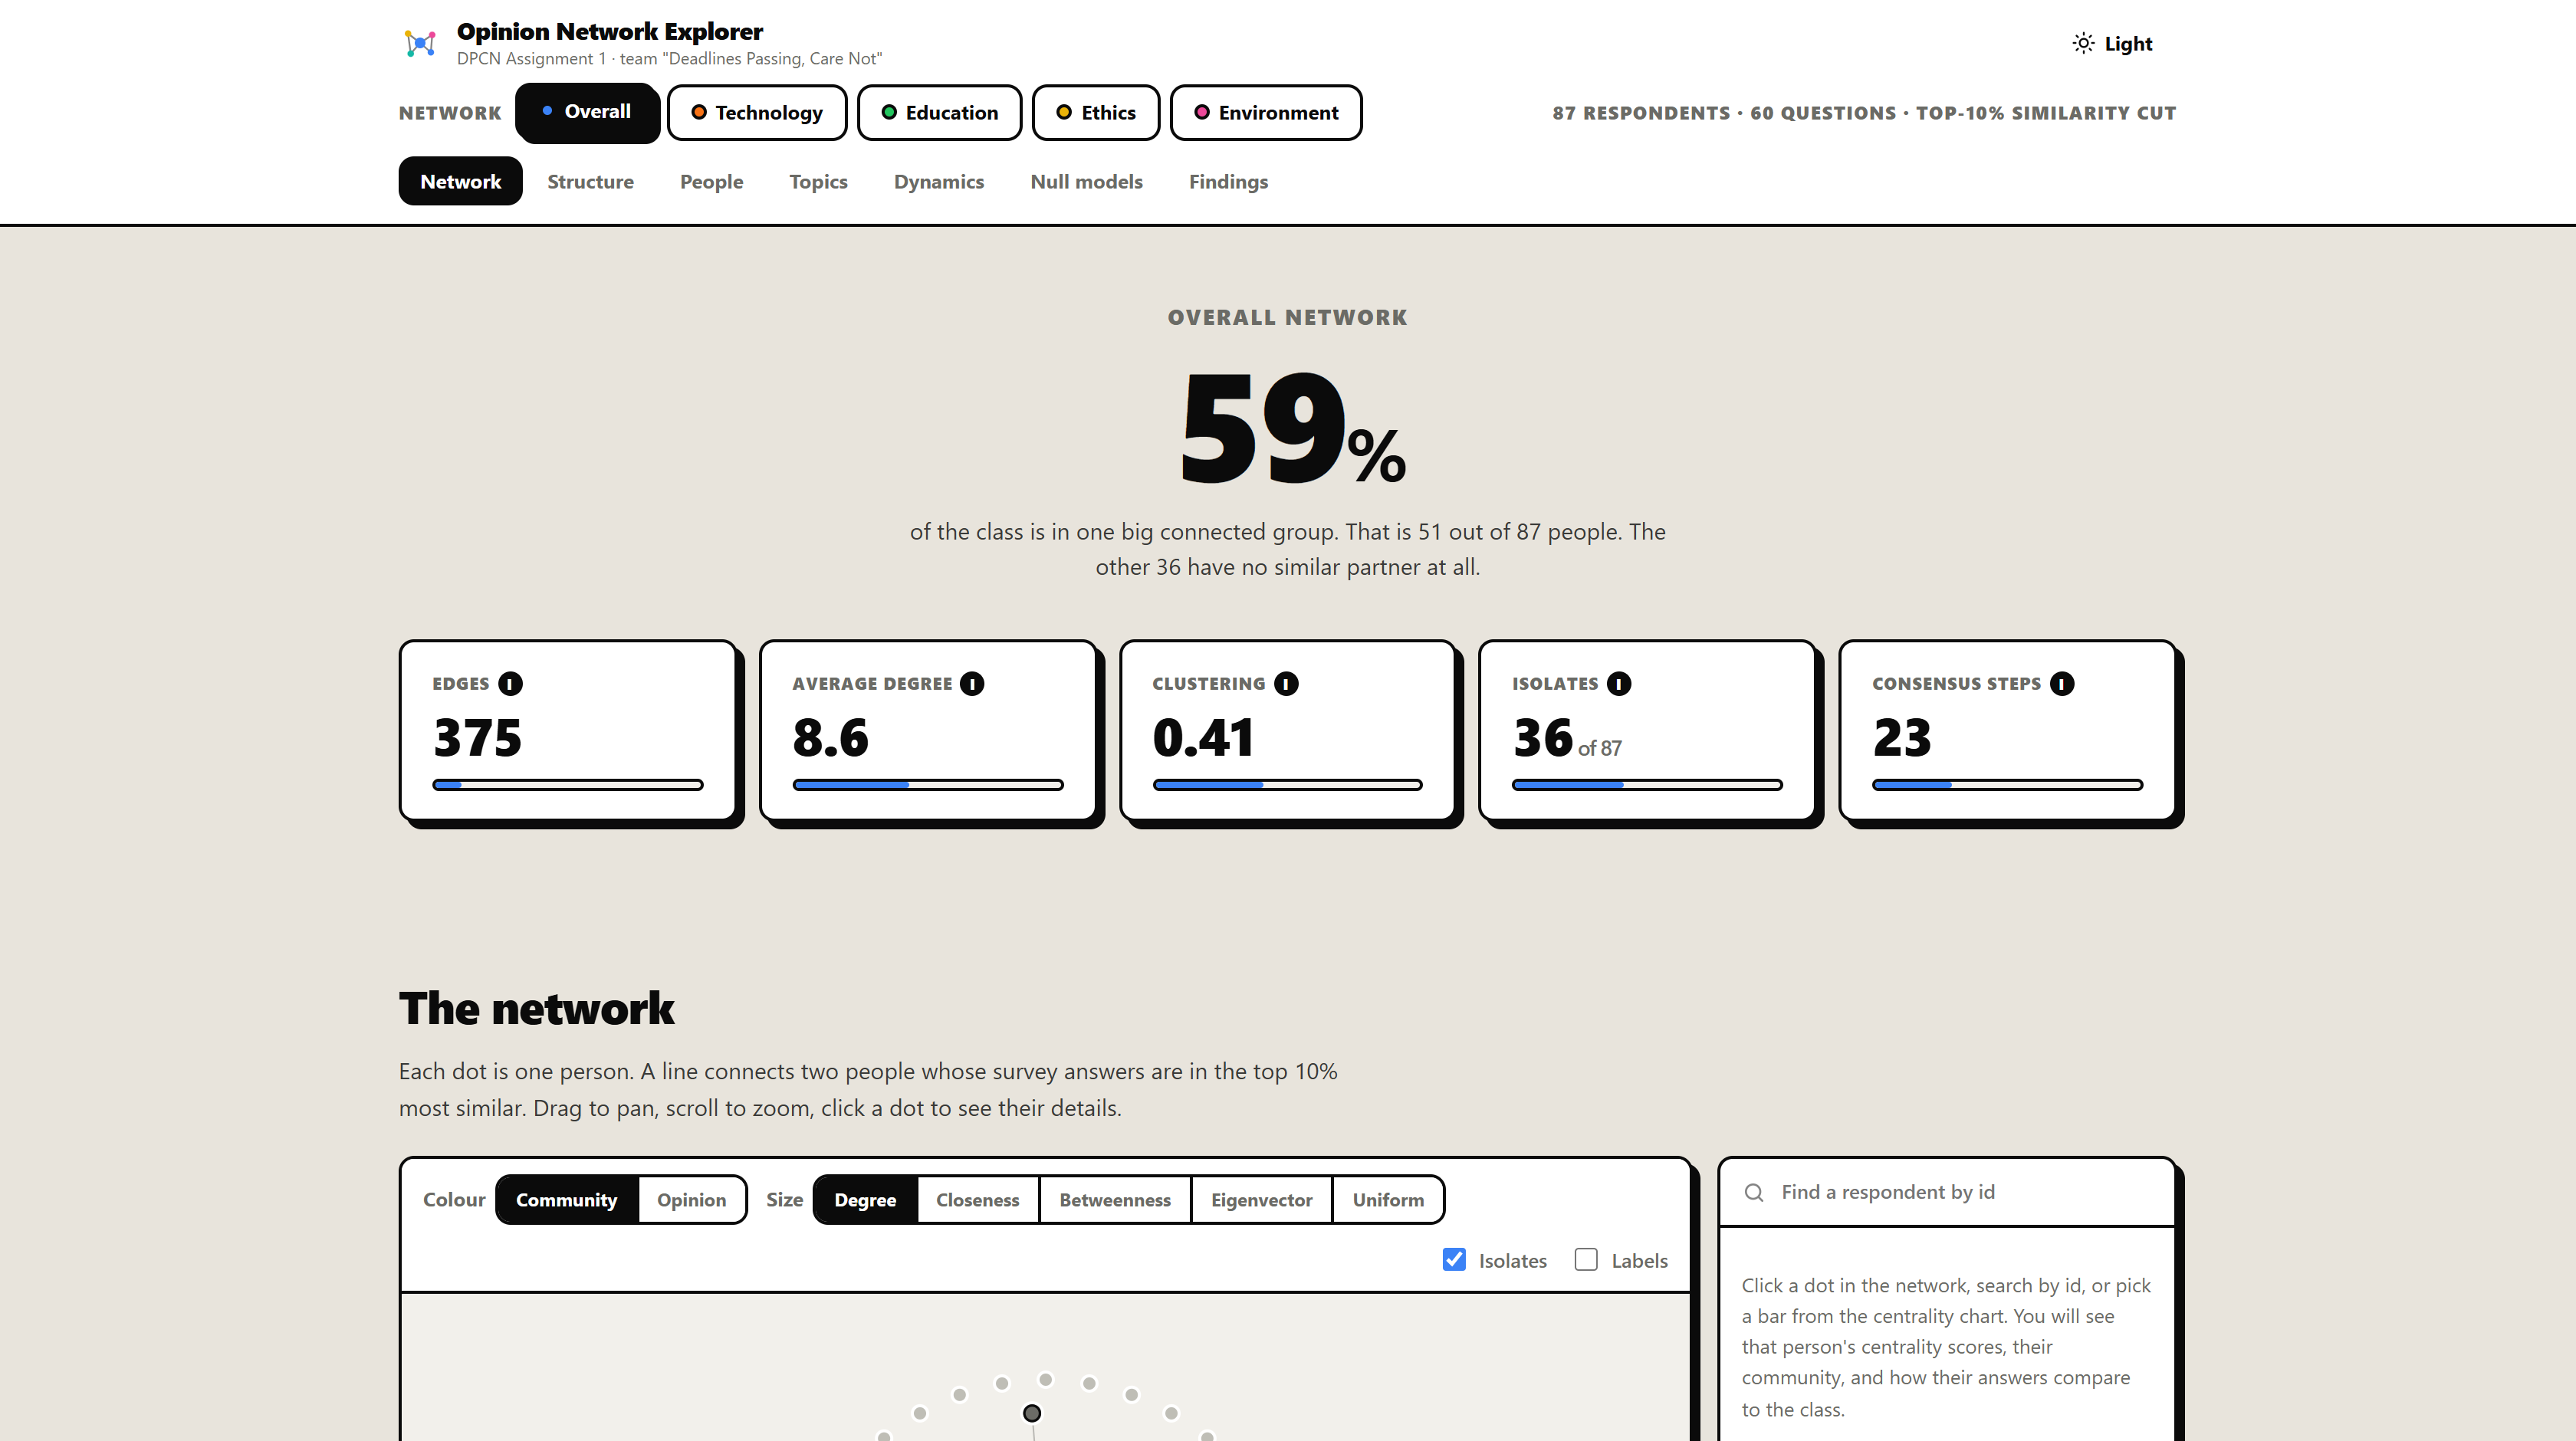
\includegraphics[width=0.90\linewidth]{../figures/dashboard/overview.png}
  \caption{The interactive dashboard. It opens in any browser and needs no
  server. The network picker changes every number, chart, and diagram to the
  chosen network.}
  \label{fig:overview}
\end{figure}

% ============================================================
\section{Dataset Documentation}

\lab{The raw survey:} 96 responses to 60 opinion statements, 15 in each of four
topics. A letter code marks the topic: \textbf{T} Technology, \textbf{E}
Education, \textbf{S} Ethics, \textbf{V} Environment. Each statement uses a
five-point Likert scale, plus a ``No Comments'' option.

\lab{Preparation:}
\begin{dash}
  \item \emph{Likert to number.} Strongly Disagree $=-2$ through Strongly Agree
  $=+2$. The scale is symmetric, so $0$ is a true neutral and a mean score
  carries a direction and a strength at once.
  \item \emph{``No Comments'' is missing, not neutral.} A refusal to answer is
  not the same as being neutral. There are 62 blanks out of $87\times60=5220$
  ($1.19\%$), spread over 19 respondents.
  \item \emph{Quality filter.} Drop any respondent who answered fewer than half
  of the 60 questions. This removes 9 responses and leaves \textbf{87
  respondents}.
  \item \emph{Result.} An $87\times60$ table of scores in $[-2,+2]$, with a blank
  for each ``No Comments''. Each question keeps its topic and its text.
\end{dash}

\lab{Missing values:} two rules are correct and both are used on purpose.
\begin{dash}
  \item Work that must agree with the graph replaces a blank with $0$ before
  averaging. This is the step the edge builder uses, so opinions and edges come
  from the same numbers.
  \item Descriptive statistics drop the blank from a person's average instead.
  \item The two rules differ by at most $0.01$ on the class mean, and by $0.23$
  for one respondent. A number from one rule is never compared with a number
  from the other.
\end{dash}

% ============================================================
\section{Pipeline Followed}

\lab{Similarity:} each respondent becomes a vector of 60 answers,
$\mathbf{x}_i\in[-2,2]^{60}$, with blanks set to $0$. The similarity of two
people is the cosine of the angle between their vectors,
\[
  s_{ij}=\frac{\mathbf{x}_i\cdot\mathbf{x}_j}
  {\lVert\mathbf{x}_i\rVert\,\lVert\mathbf{x}_j\rVert}\in[-1,1].
\]
The cosine rewards a shared pattern across all 60 questions. It does not reward
a shared average level alone.

\lab{Edges:} compute the full $87\times87$ cosine matrix, then keep the top
\textbf{10\%} of pairs as edges. That is the 90th-percentile cut.
\begin{dash}
  \item A hard cut is necessary. Almost everyone in this class agrees on
  average, so a loose threshold gives a near-complete graph with no information.
  \item The rule keeps a fixed \emph{rank}, not a fixed score. It therefore
  yields exactly \textbf{375 edges} every time, whatever the similarity
  distribution looks like.
  \item \textbf{Five networks} use the same rule. One \emph{overall} network uses
  all 60 questions. Four use one topic each, 15 questions apiece.
  \item Because node count, edge count, and density are identical across the
  five, any difference between them is a wiring effect. Section~\ref{sec:sens}
  tests the cut itself.
\end{dash}

\begin{figure}[htbp]
\centering
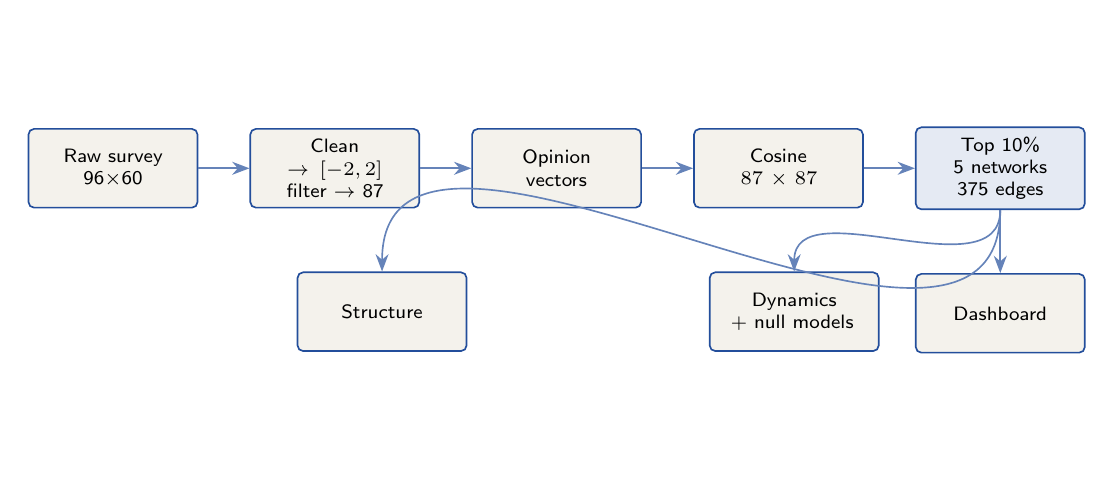
\begin{tikzpicture}[
  node distance=6mm and 6.5mm,
  box/.style={rectangle, rounded corners=2pt, draw=accent, line width=0.6pt,
    fill=soft, align=center, font=\sffamily\scriptsize, inner sep=3.5pt,
    text width=19mm, minimum height=10mm},
  outb/.style={box, fill=accent!12},
  ar/.style={-{Stealth[length=2.2mm]}, line width=0.6pt, draw=accent!70}]
\node[box] (raw) {Raw survey\\96$\times$60};
\node[box, right=of raw] (clean) {Clean\\$\to[-2,2]$\\filter $\to$ 87};
\node[box, right=of clean] (vec) {Opinion\\vectors};
\node[box, right=of vec] (sim) {Cosine\\$87\times87$};
\node[outb, right=of sim] (net) {Top 10\%\\5 networks\\375 edges};
\draw[ar] (raw)--(clean); \draw[ar] (clean)--(vec);
\draw[ar] (vec)--(sim); \draw[ar] (sim)--(net);
\node[box, below=8mm of clean, xshift=6mm] (struct) {Structure};
\node[box, below=8mm of sim, xshift=2mm] (dyn) {Dynamics\\+ null models};
\node[box, below=8mm of net] (dash) {Dashboard};
\draw[ar] (net.south) to[out=-90,in=90] (struct.north);
\draw[ar] (net.south) to[out=-90,in=90] (dyn.north);
\draw[ar] (net.south) -- (dash.north);
\end{tikzpicture}
\caption{The pipeline. Clean the survey, build the opinion vectors, compute the
cosine matrix, cut the top 10\% of pairs into five networks. Structure,
dynamics, and dashboard all read those saved networks. No later stage rebuilds
the graph.}
\label{fig:pipe}
\end{figure}

% ============================================================
\section{Analysis and Visualizations}
\label{sec:analysis}

\subsection{Structure}

\lab{Definitions:} \emph{degree} $k$ is the number of edges at a node.
\emph{Density} is the fraction of possible edges present. \emph{Clustering}
measures how often two neighbours of a node also connect to each other, on a
scale of $0$ to $1$. A \emph{component} is a set of nodes that can all reach each
other, and the largest one is the \emph{giant component}. \emph{Modularity} $Q$
scores a grouping by how many more edges fall inside groups than a random graph
with the same degrees would give.

\lab{Results:}

\begin{table}[htbp]
\centering\small
\begin{tabular}{@{}lrrrrr@{}}
\toprule
\sffamily\bfseries Metric & \sffamily Overall & \sffamily Technology &
\sffamily Education & \sffamily Ethics & \sffamily Environment \\
\midrule
Nodes / Edges        & 87 / 375 & 87 / 375 & 87 / 375 & 87 / 375 & 87 / 375 \\
Density              & 0.100 & 0.100 & 0.100 & 0.100 & 0.100 \\
Avg.\ degree $\langle k\rangle$ & 8.62 & 8.62 & 8.62 & 8.62 & 8.62 \\
Avg.\ clustering     & \gc{0.408} & 0.387 & 0.396 & \rc{0.363} & 0.375 \\
Components           & 37 & \gc{21} & 23 & 42 & \rc{43} \\
Giant component      & 58.6\% & \gc{74.7\%} & 72.4\% & 51.7\% & \rc{50.6\%} \\
Giant diameter       & 4 & 5 & 6 & 4 & 5 \\
Giant avg.\ path     & 1.88 & 2.20 & 2.24 & 1.78 & 1.93 \\
Modularity $Q$       & 0.108 & 0.242 & \gc{0.263} & 0.151 & \rc{0.079} \\
\bottomrule
\end{tabular}
\caption{Structural metrics per network. Node count, edge count, and density are
identical by construction, so every other difference is an opinion effect.}
\label{tab:struct}
\end{table}

\lab{Analysis:}
\begin{dash}
  \item The overall network is sparse but locally dense. Density is $0.10$ and
  clustering is $0.41$. Connected people sit in tight triangles.
  \item \textbf{36 of 87 respondents are isolates.} An isolate has no
  strong-similarity partner anywhere in the class.
  \item The giant component is compact. Two connected people are $1.88$ steps
  apart on average, with a diameter of $4$.
  \item The degree distribution is heavy-tailed. Respondent 114 has $k=35$ while
  the mean is $8.6$, a value that fits almost nobody
  (Figure~\ref{fig:structure}).
\end{dash}

\begin{figure}[htbp]
  \centering
  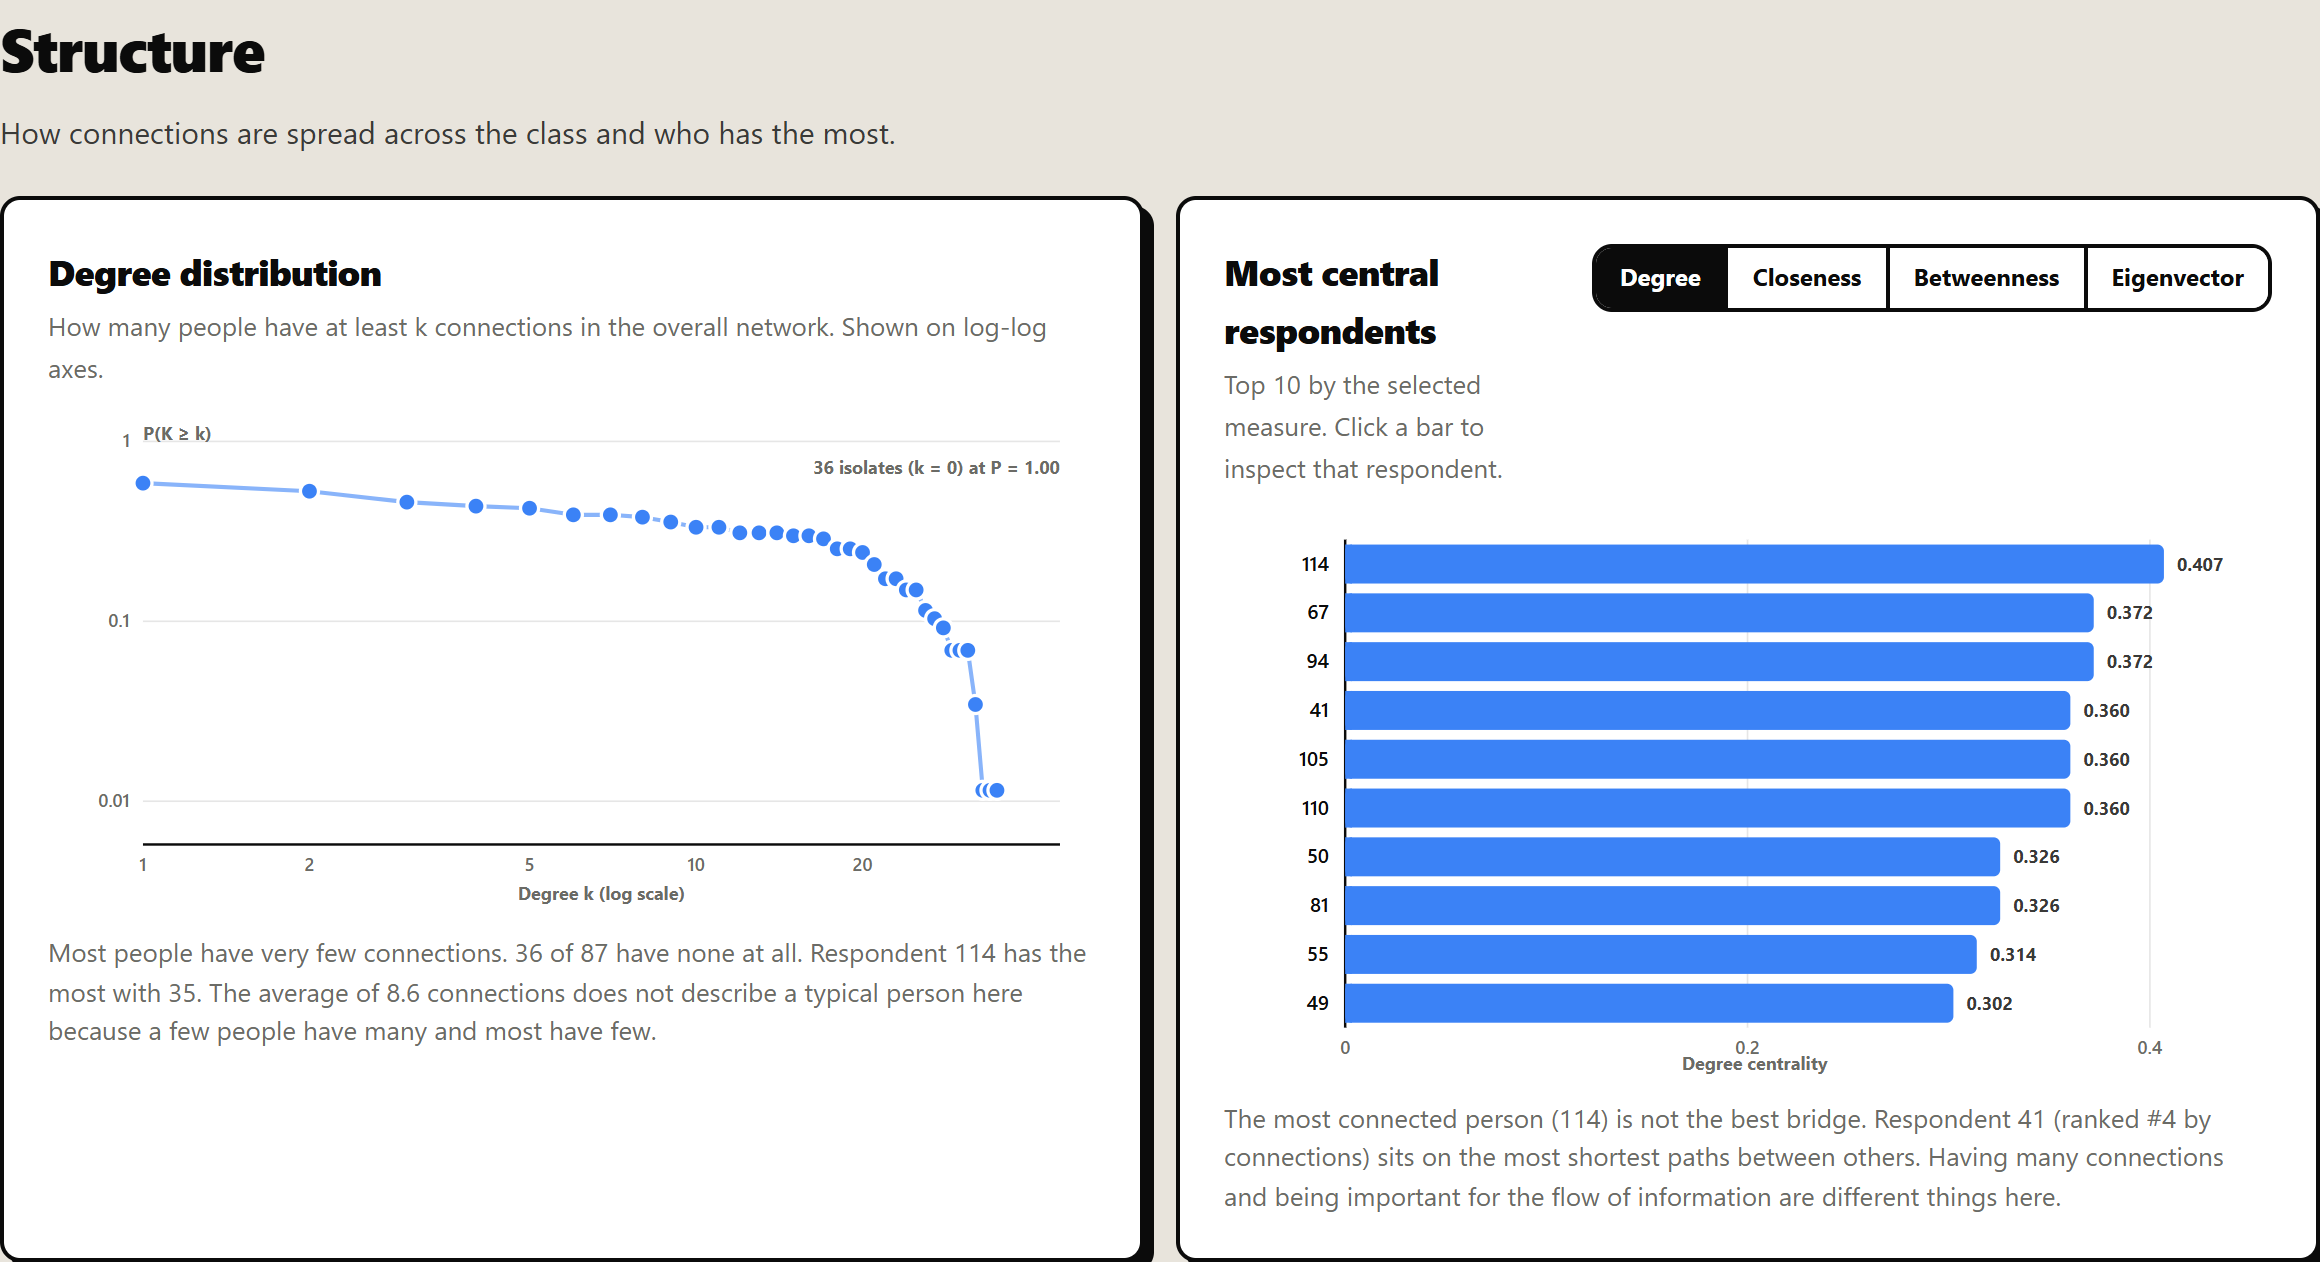
\includegraphics[width=\linewidth]{../figures/dashboard/structure.png}
  \caption{\emph{Left:} degree distribution on log-log axes as a complementary
  CDF $P(K\ge k)$. The 36 isolates sit at $k=0$, which a log axis cannot draw, so
  the chart states this rather than dropping them silently. \emph{Right:} the ten
  most central respondents by degree.}
  \label{fig:structure}
\end{figure}

\subsection{Centrality and communities}

\lab{Definitions:} \emph{degree} centrality counts direct connections.
\emph{Closeness} measures how short the average path is to everyone else.
\emph{Betweenness} counts how often a node lies on a shortest path between two
others, which rewards a bridge position. \emph{Eigenvector} centrality gives more
weight to a node connected to other important nodes. \emph{Louvain} searches for
the grouping with the highest modularity.

\lab{Analysis:}
\begin{dash}
  \item Degree, closeness, and eigenvector centrality pick almost the same five
  people: 114, 67, 94, 105, 110. All five score above the class mean on every
  topic. They are the uniform strong-agreement answerers, so their 60-value
  vectors resemble many others.
  \item Betweenness gives a different answer. Its top node is \textbf{41}, who has
  a maximum Technology score but only an average Education score. That mixed
  profile bridges sub-groups.
  \item The most connected person and the best bridge are different people. One
  centrality measure is not enough to describe importance here.
  \item Louvain finds many small communities and a low modularity
  ($Q=0.108$). Every community has a positive mean on every topic. Only one group
  (C6) falls below the class mean anywhere, and only on Technology. These are
  degrees of agreement, not opposing camps.
\end{dash}

\begin{figure}[htbp]
  \centering
  \begin{subfigure}{0.485\linewidth}
    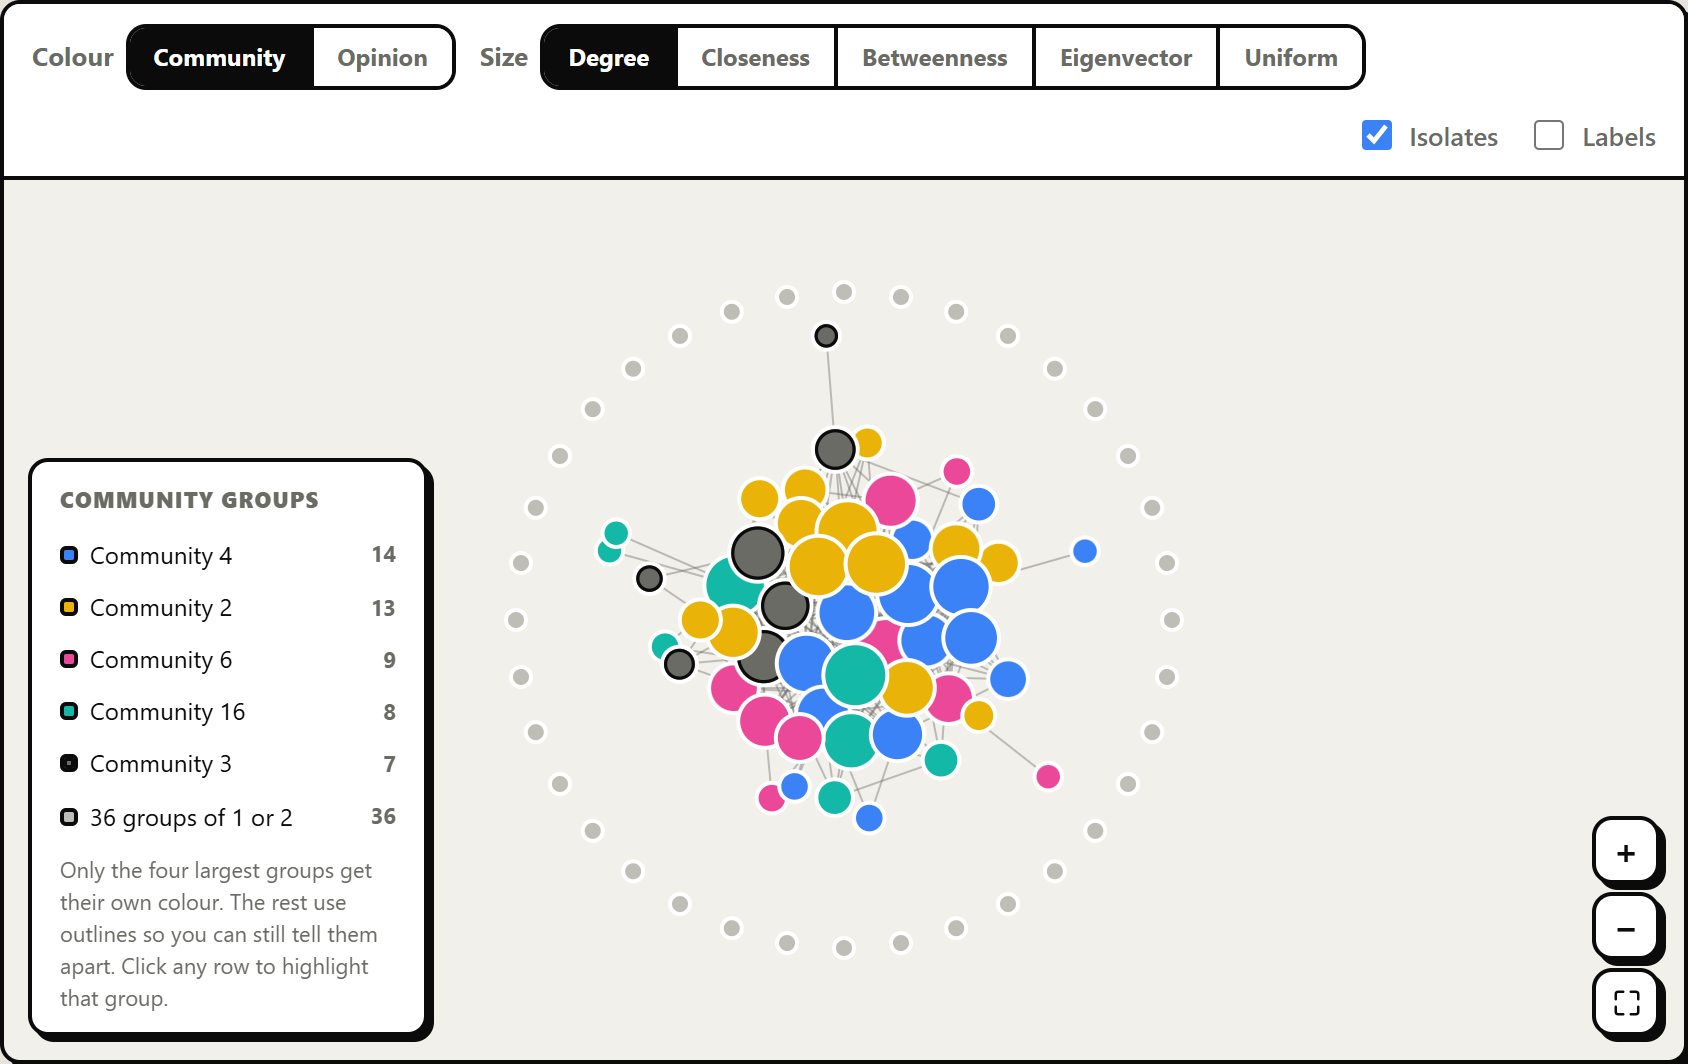
\includegraphics[width=\linewidth]{../figures/dashboard/network_overall_community.png}
    \caption{Overall, coloured by community.}
  \end{subfigure}\hfill
  \begin{subfigure}{0.485\linewidth}
    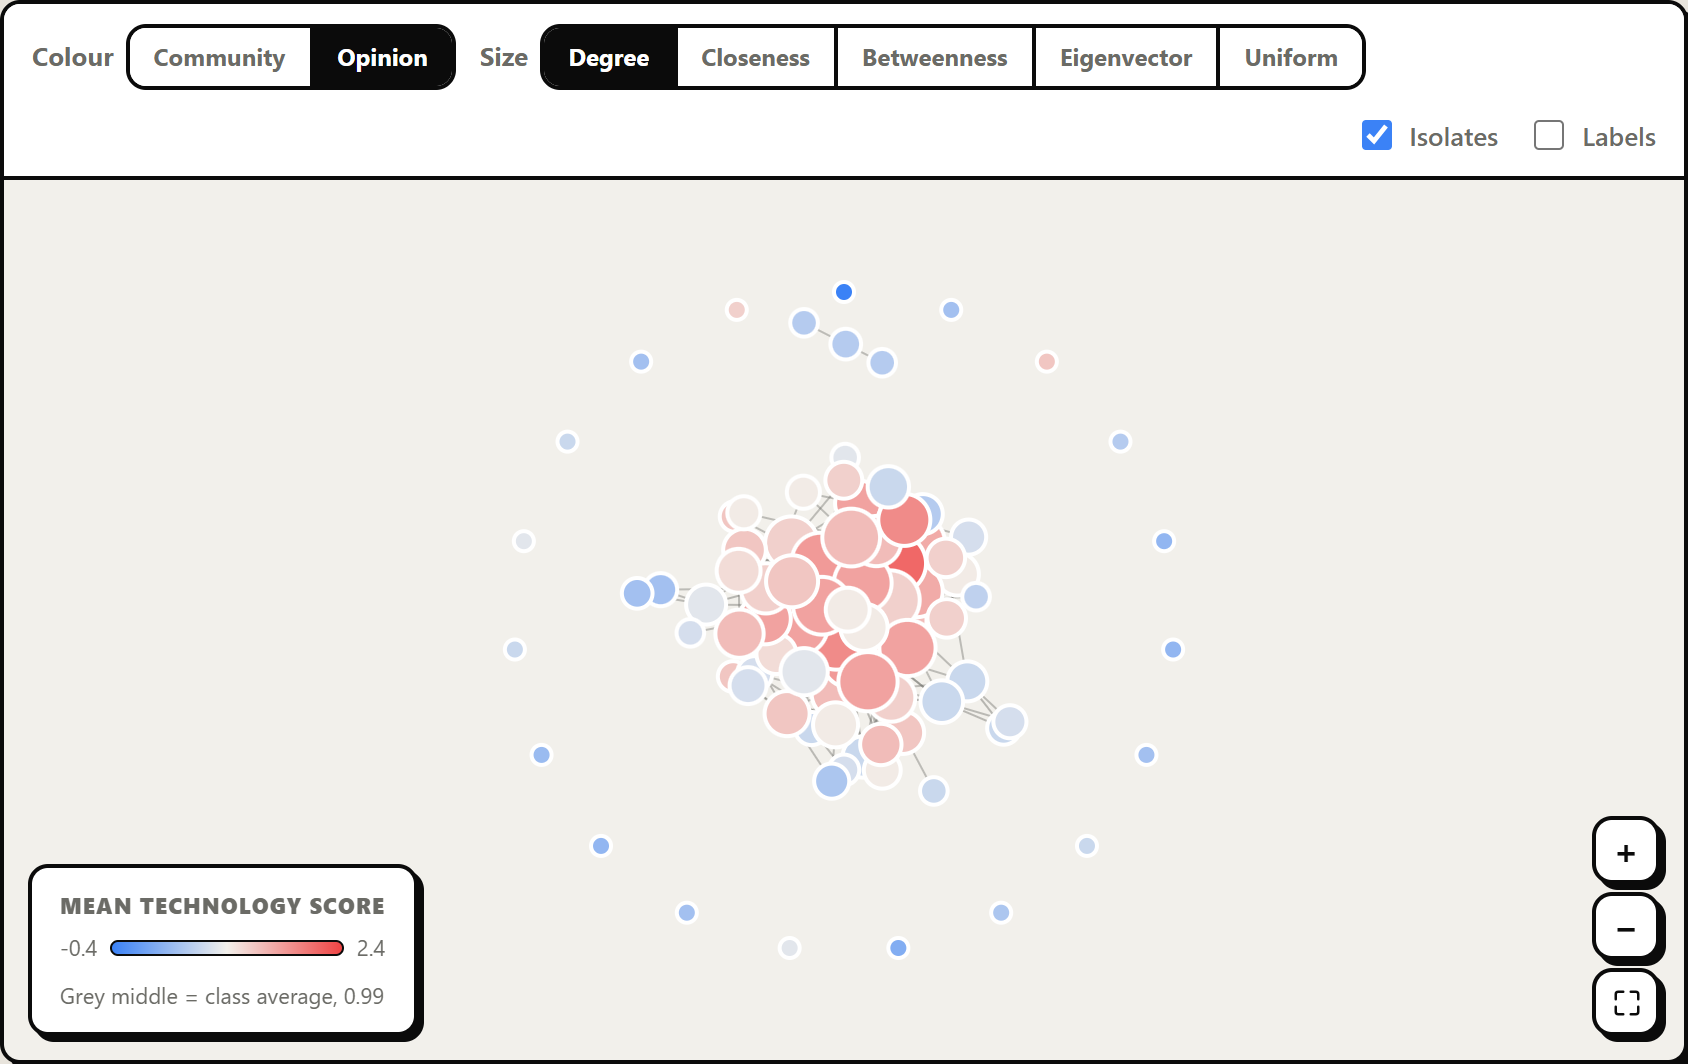
\includegraphics[width=\linewidth]{../figures/dashboard/network_technology_opinion.png}
    \caption{Technology, coloured by opinion.}
  \end{subfigure}
  \caption{Node-link view, node size scaled by degree. The giant component sits
  in the centre, small components ring it, isolates sit on the outer rim.
  \textbf{(a)} The four largest Louvain communities are coloured, singletons and
  pairs are grey. \textbf{(b)} Strong-agreement answerers (red) form the centre;
  lukewarm answerers (blue) sit on the edge.}
  \label{fig:nets}
\end{figure}

\subsection{Cohesion tracks opinion variance, not opinion strength}

\lab{Observation:} the per-topic numbers run against the raw averages.

\begin{table}[htbp]
\centering\small
\begin{tabular}{@{}lrrrr@{}}
\toprule
\sffamily\bfseries Topic & \sffamily Class mean & \sffamily Std.\ dev. &
\sffamily Giant component & \sffamily Components \\
\midrule
Technology  & 0.99 & \gc{0.37} & \gc{74.7\%} & \gc{21} \\
Education   & \rc{0.91} & \gc{0.35} & 72.4\% & 23 \\
Ethics      & 1.28 & 0.45 & 51.7\% & 42 \\
Environment & \gc{1.37} & \rc{0.47} & \rc{50.6\%} & \rc{43} \\
\bottomrule
\end{tabular}
\caption{The topics with the strongest average agreement have the most broken
networks. The spread explains it, not the mean.}
\label{tab:variance}
\end{table}

\lab{Analysis:}
\begin{dash}
  \item Ethics ($+1.28$) and Environment ($+1.37$) have the strongest average
  agreement, yet the most broken networks at $52\%$ and $51\%$.
  \item Technology ($+0.99$) and Education ($+0.91$) agree less on average, yet
  stay the best connected at $75\%$ and $72\%$.
  \item The cause is the spread. Cosine similarity depends on the pattern across
  the 15 questions of a topic, not on the average level.
  \item Technology and Education opinions are tightly grouped (s.d.\ $0.37$ and
  $0.35$), so most vectors stay similar and the graph holds together. Ethics and
  Environment are strong but spread out (s.d.\ $0.45$ and $0.47$), so the same
  cut fragments them.
  \item ``The class agrees more on Environment than on Technology'' is true of
  the raw average and false of the network.
\end{dash}

\subsection{Dynamics on the network}

\lab{DeGroot:} give each respondent a start opinion, their mean score. At each
step every respondent replaces it with the mean of their neighbours' opinions,
all at the same time. The rule is $\mathbf{x}(t{+}1)=D^{-1}A\,\mathbf{x}(t)$.
The eigenvalues of the update matrix decide the outcome. The course stability
rule says a linear map is stable when the relevant eigenvalue has magnitude below
$1$. The \emph{SLEM} (second-largest eigenvalue modulus) sets the speed, and the
algebraic connectivity is $\lambda_2=1-\mu_2$.

\lab{Results:}

\begin{table}[htbp]
\centering\small
\begin{tabular}{@{}lrrrrr@{}}
\toprule
\sffamily\bfseries Network & \sffamily $\lambda_2$ & \sffamily SLEM &
\sffamily Steps & \sffamily Core size & \sffamily Consensus \\
\midrule
Overall     & \gc{0.627} & \gc{0.397} & \gc{23} & 51 & 1.409 \\
Ethics      & 0.455 & 0.545 & 31 & 45 & 1.350 \\
Technology  & 0.318 & 0.682 & 53 & \gc{65} & 1.313 \\
Education   & 0.264 & 0.736 & 61 & 63 & \rc{1.275} \\
Environment & \rc{0.229} & \rc{0.771} & \rc{77} & \rc{44} & 1.349 \\
\bottomrule
\end{tabular}
\caption{DeGroot consensus. Every SLEM is below $1$, so every map is stable. The
order of $\lambda_2$ matches the order of the measured steps with no exception.}
\label{tab:degroot}
\end{table}

\lab{Analysis:}
\begin{dash}
  \item The overall network has 37 components, so there is no single class
  consensus. The 51-person core reaches \textbf{1.409} in \textbf{23 steps}.
  \item The 36 isolates never move. An isolate has no neighbour to average with,
  so its opinion at step 1000 equals its opinion at step 0.
  \item Convergence speed follows the algebraic connectivity exactly across all
  five networks. This is the course stability rule confirmed on survey data.
  \item Edge weights have almost no effect. The weighted consensus is $1.4099$
  against an unweighted $1.4085$. Row normalisation removes the narrow $0.85$ to
  $0.95$ range of the kept similarities.
\end{dash}

\lab{SIS:} model a strong opinion as a contagion. An infected person infects each
neighbour at rate $\beta$ and recovers at rate $\gamma$. The course result gives a
critical ratio $(\beta/\gamma)_c = 1/\lambda_{\max}$, where $\lambda_{\max}$ is
the largest eigenvalue of the adjacency matrix. A lower threshold means an opinion
spreads more easily. Note this uses $A$ itself, not the row-normalised $D^{-1}A$,
because an infected person infects each neighbour separately rather than
averaging.

\begin{figure}[htbp]
  \centering
  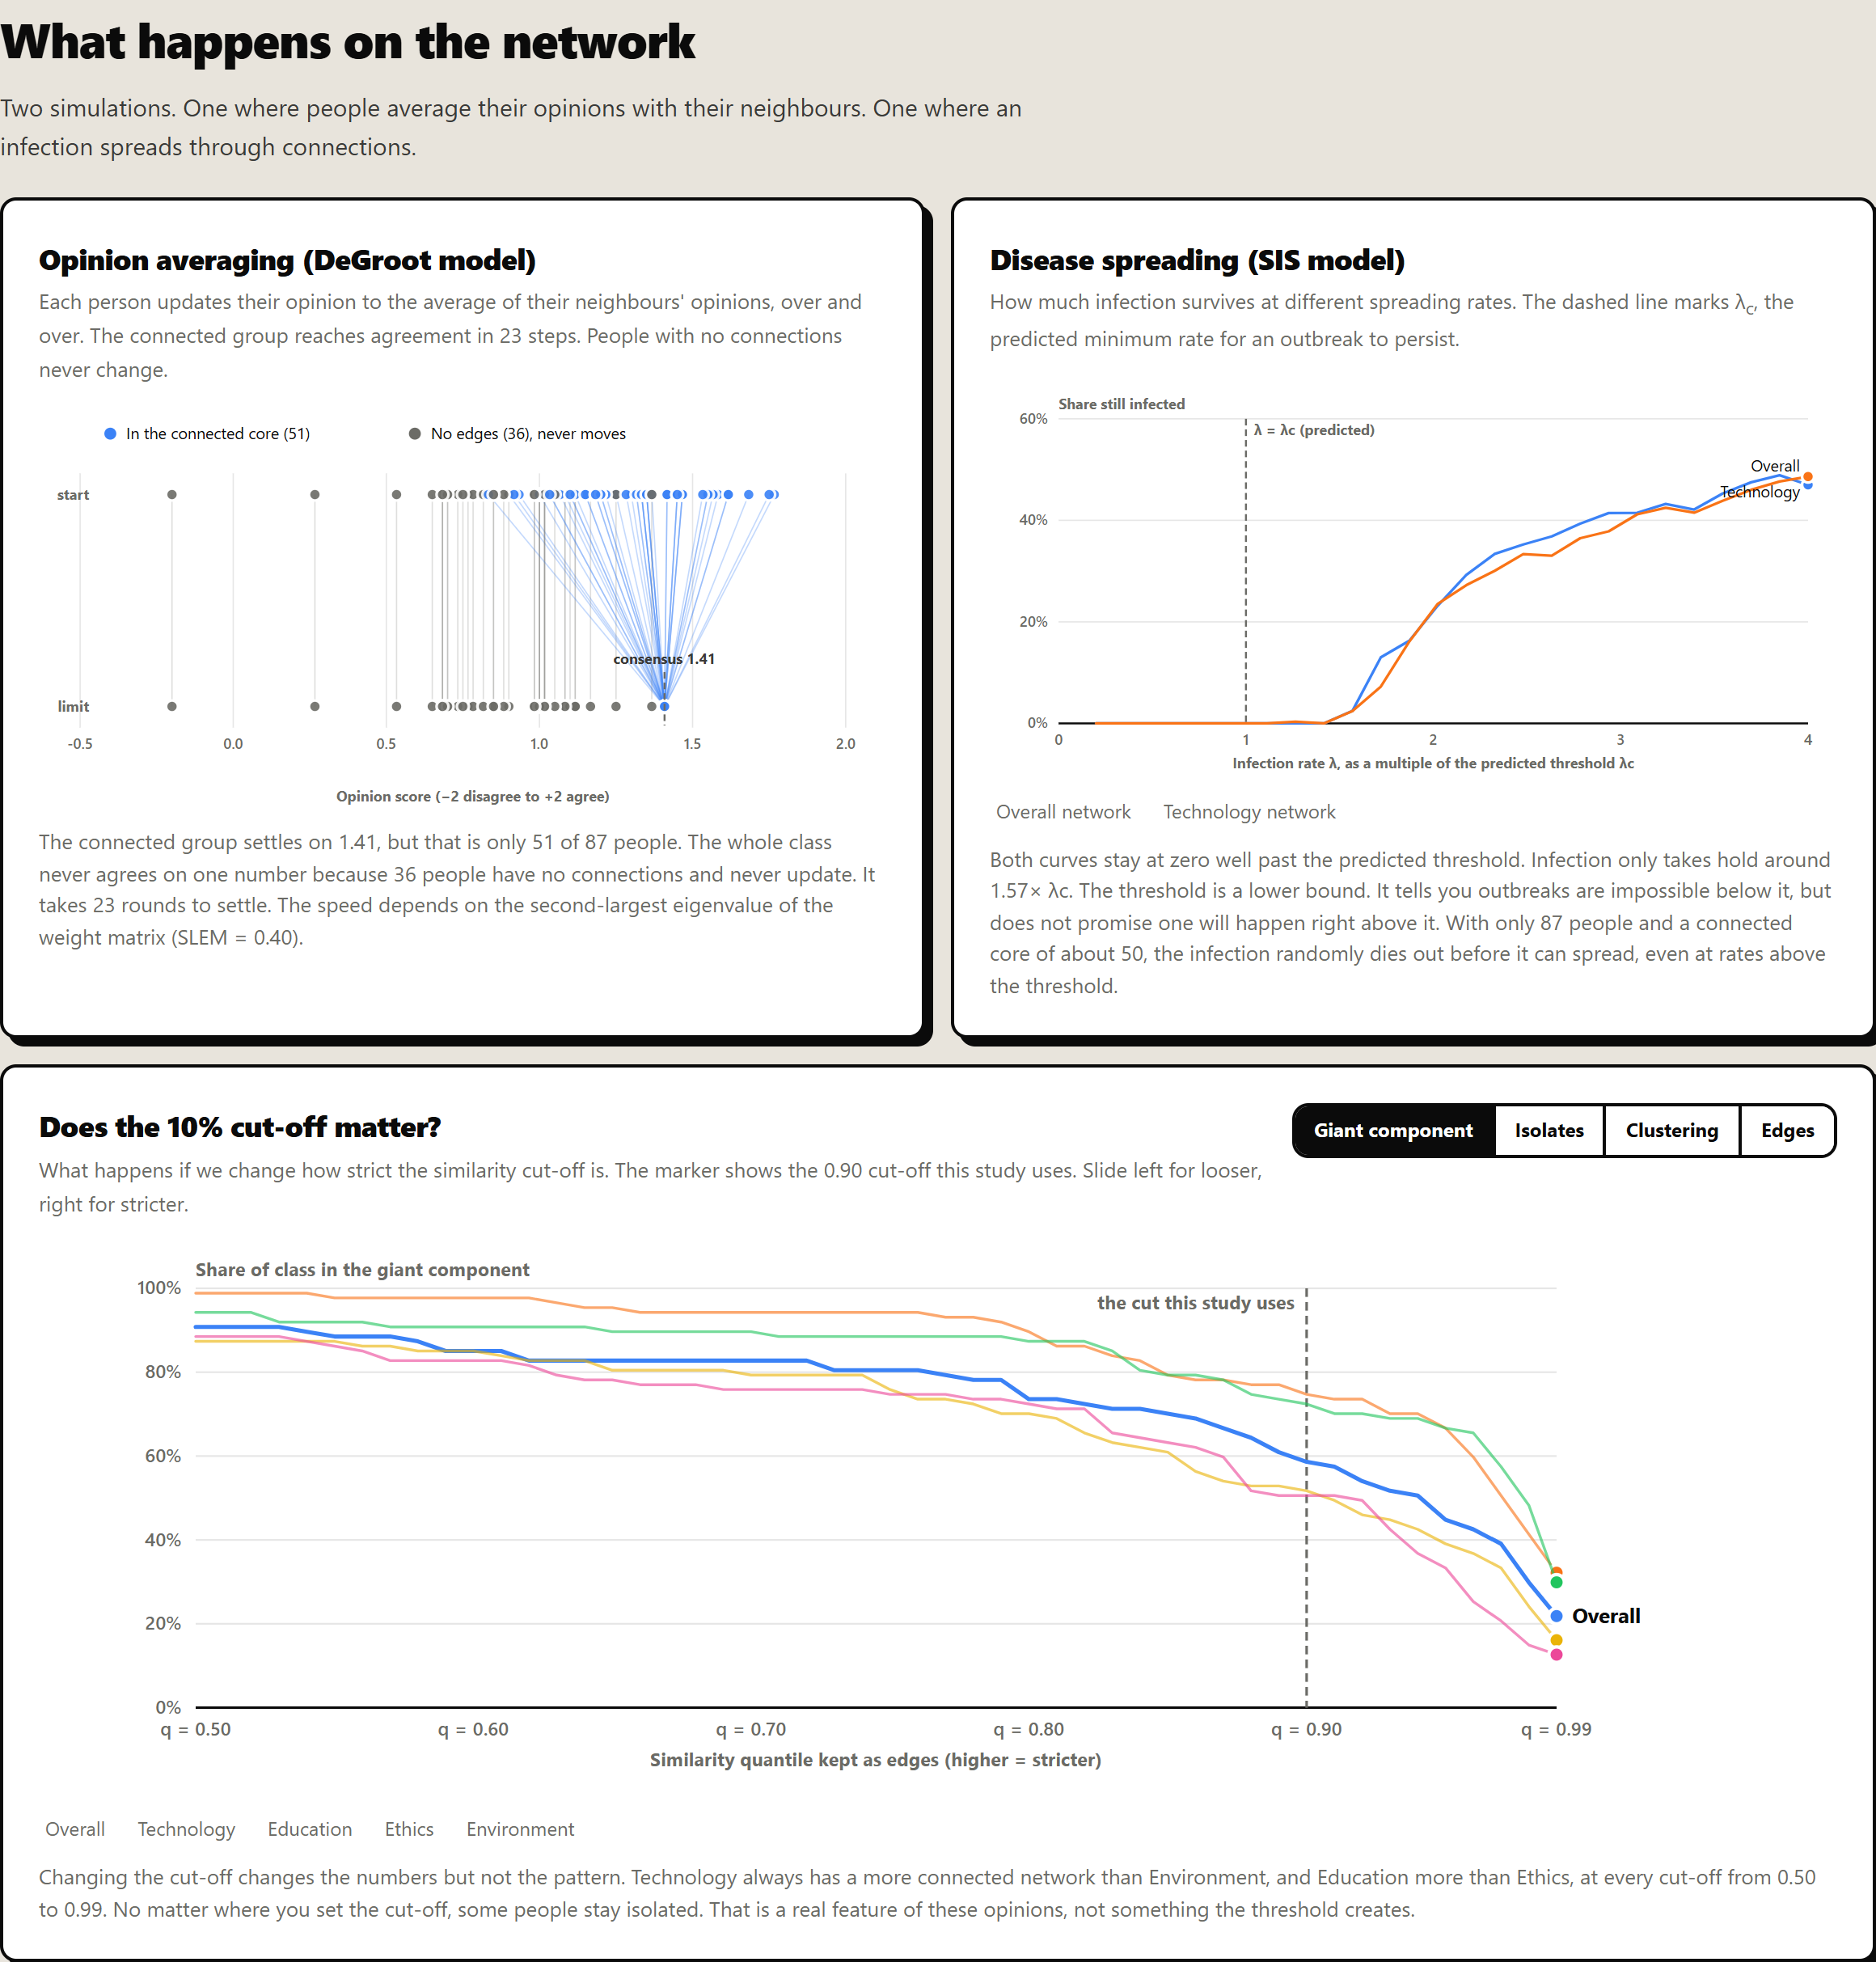
\includegraphics[width=0.78\linewidth]{../figures/dashboard/dynamics.png}
  \caption{\emph{Left:} DeGroot. The connected core funnels onto $1.41$ while the
  isolate lines stay flat. \emph{Right:} the simulated SIS transition begins at
  about $1.6\times$ the predicted bound, which is expected because the mean-field
  value is a lower bound and the core holds only 44 to 65 people.
  \emph{Bottom:} the threshold sensitivity sweep.}
  \label{fig:dynamics}
\end{figure}

\subsection{Does the 10\% cut-off matter?}
\label{sec:sens}

\lab{Experiment:} apply the same rule at every quantile from $0.50$ to $0.99$ and
record the structure at each one.

\lab{Results:}

\begin{table}[htbp]
\centering\small
\begin{tabular}{@{}lrrrr@{}}
\toprule
\sffamily\bfseries Quantile kept & \sffamily Edges & \sffamily Isolates &
\sffamily Giant component & \sffamily Clustering \\
\midrule
0.90 (used) & 375  & \rc{36} & \rc{58.6\%} & \gc{0.408} \\
0.80        & 749  & 21 & 73.6\% & 0.579 \\
0.70        & 1123 & 15 & 82.8\% & 0.643 \\
0.60        & 1497 & 13 & 85.1\% & 0.674 \\
0.50        & 1871 & \gc{8}  & \gc{90.8\%} & \rc{0.751} \\
\bottomrule
\end{tabular}
\caption{Loosening the cut connects most of the isolates but never all of them,
and inflates the clustering until the graph stops being informative.}
\label{tab:sens}
\end{table}

\lab{Analysis:}
\begin{dash}
  \item The topic order is stable at every cut. Technology stays above
  Environment and Education stays above Ethics, with no exception. That order is
  a property of the data, not of the 90th percentile.
  \item The isolates are only partly an artifact. Their count falls from 36 at
  $q=0.90$ to 8 at $q=0.50$, and never reaches zero. Eight people stay below the
  median similarity to every other person in the class.
  \item A looser cut has a cost. At $q=0.50$ the clustering rises to $0.75$ and
  the graph is half complete, so community detection and centrality stop meaning
  much.
  \item $q=0.90$ is therefore a tested compromise rather than an assumption.
\end{dash}

% ============================================================
\section{Results and Discussion}
\label{sec:results}

\lab{What the network says about class opinions:} this class is agreeable. The
mean opinion is positive on all four topics and the raw data shows no opposing
camps. The network exposes structure that the averages hide.

\lab{Finding 1. No global consensus, and the drop-outs are the moderates.}
\begin{dash}
  \item Under DeGroot the 51-person core agrees at $1.409$ while the 36 isolates
  never move.
  \item The core started at a mean of $1.309$. The isolates started at $0.872$.
  \item So the process removes the more moderate half of the class. This is a
  structural effect of the construction, not something the averaging model
  causes.
\end{dash}

\lab{Finding 2. Cohesion is a variance story.} Technology and Education look
better connected than Ethics and Environment despite lower mean scores, because
their opinions are less spread out. Raw agreement and social cohesion are not the
same measurement.

\lab{Finding 3. Spread is easiest where the class is most broken.}

\begin{table}[htbp]
\centering\small
\begin{tabular}{@{}lrrrr@{}}
\toprule
\sffamily\bfseries Network & \sffamily $\lambda_{\max}$ &
\sffamily $1/\lambda_{\max}$ & \sffamily Giant size & \sffamily Giant density \\
\midrule
Environment & \gc{23.92} & \gc{0.0418} & \rc{44} & \gc{0.395} \\
Ethics      & 22.45 & 0.0445 & 45 & 0.378 \\
Overall     & 22.06 & 0.0453 & 51 & 0.294 \\
Technology  & 18.17 & 0.0550 & \gc{65} & 0.179 \\
Education   & \rc{17.74} & \rc{0.0564} & 63 & \rc{0.191} \\
\bottomrule
\end{tabular}
\caption{Epidemic thresholds. The order reverses the connectivity order in
Table~\ref{tab:struct}. The most broken topic spreads most easily.}
\label{tab:epi}
\end{table}

\begin{dash}
  \item Environment and Ethics have the lowest thresholds at $0.0418$ and
  $0.0445$, yet they are the least connected topics.
  \item The edge count is fixed at 375, so a smaller giant component packs almost
  the same edges into fewer people. Environment puts 374 edges into 44
  respondents; Technology spreads 373 across 65.
  \item A denser core raises $\lambda_{\max}$, which lowers the threshold. The
  standard bound $\langle k\rangle \le \lambda_{\max} \le k_{\max}$ applied inside
  the giant component predicts this ordering directly.
  \item Fragmentation and easy spread are not opposites here. This is a real
  property of the data and also a warning about the fixed-edge method.
\end{dash}

\lab{Finding 4. The structure is in the degree sequence.} A null model asks
whether a random network with no opinion structure gives the same value. The
z-score is $z=(\text{real}-\text{null mean})/\text{null s.d.}$, and $|z|<2$ means
the real value looks random.

\begin{table}[htbp]
\centering\small
\begin{tabular}{@{}lrrrrr@{}}
\toprule
\sffamily\bfseries Statistic & \sffamily Real & \sffamily ER mean &
\sffamily $z$ & \sffamily Rewired mean & \sffamily $z$ \\
\midrule
Average clustering  & 0.408 & 0.098 & \rc{$+27.2$} & 0.391 & \gc{$+1.6$} \\
Giant fraction      & 0.586 & 1.000 & \rc{$-361.7$} & 0.586 & \gc{$0.0$} \\
Average path length & 1.880 & 2.292 & \rc{$-9.5$} & 1.834 & $+3.7$ \\
Modularity          & 0.105 & 0.282 & \rc{$-13.7$} & 0.100 & \gc{$+0.9$} \\
\bottomrule
\end{tabular}
\caption{The real network against 500 Erd\H{o}s--R\'enyi graphs of the same
density and 500 degree-preserving rewirings of itself. Green marks a z-score
inside the random band.}
\label{tab:null}
\end{table}

\begin{dash}
  \item Against 500 ER graphs the network is unusual on every measure, with a
  clustering z-score of $+27$ and a giant-fraction z-score of $-362$.
  \item Against 500 degree-preserving rewirings it is ordinary. Clustering, giant
  component, and modularity all fall inside $|z|<2$.
  \item So once each person's edge count is fixed, chance supplies the rest of
  the structure.
  \item For this construction that is the same statement as ``the connected core
  is the group that agrees with everything''. Agreement level sets the degree, and
  after the degrees are fixed nothing is left to explain. This gives the reason
  for the structural analysis rather than weakening it.
\end{dash}

\begin{figure}[htbp]
  \centering
  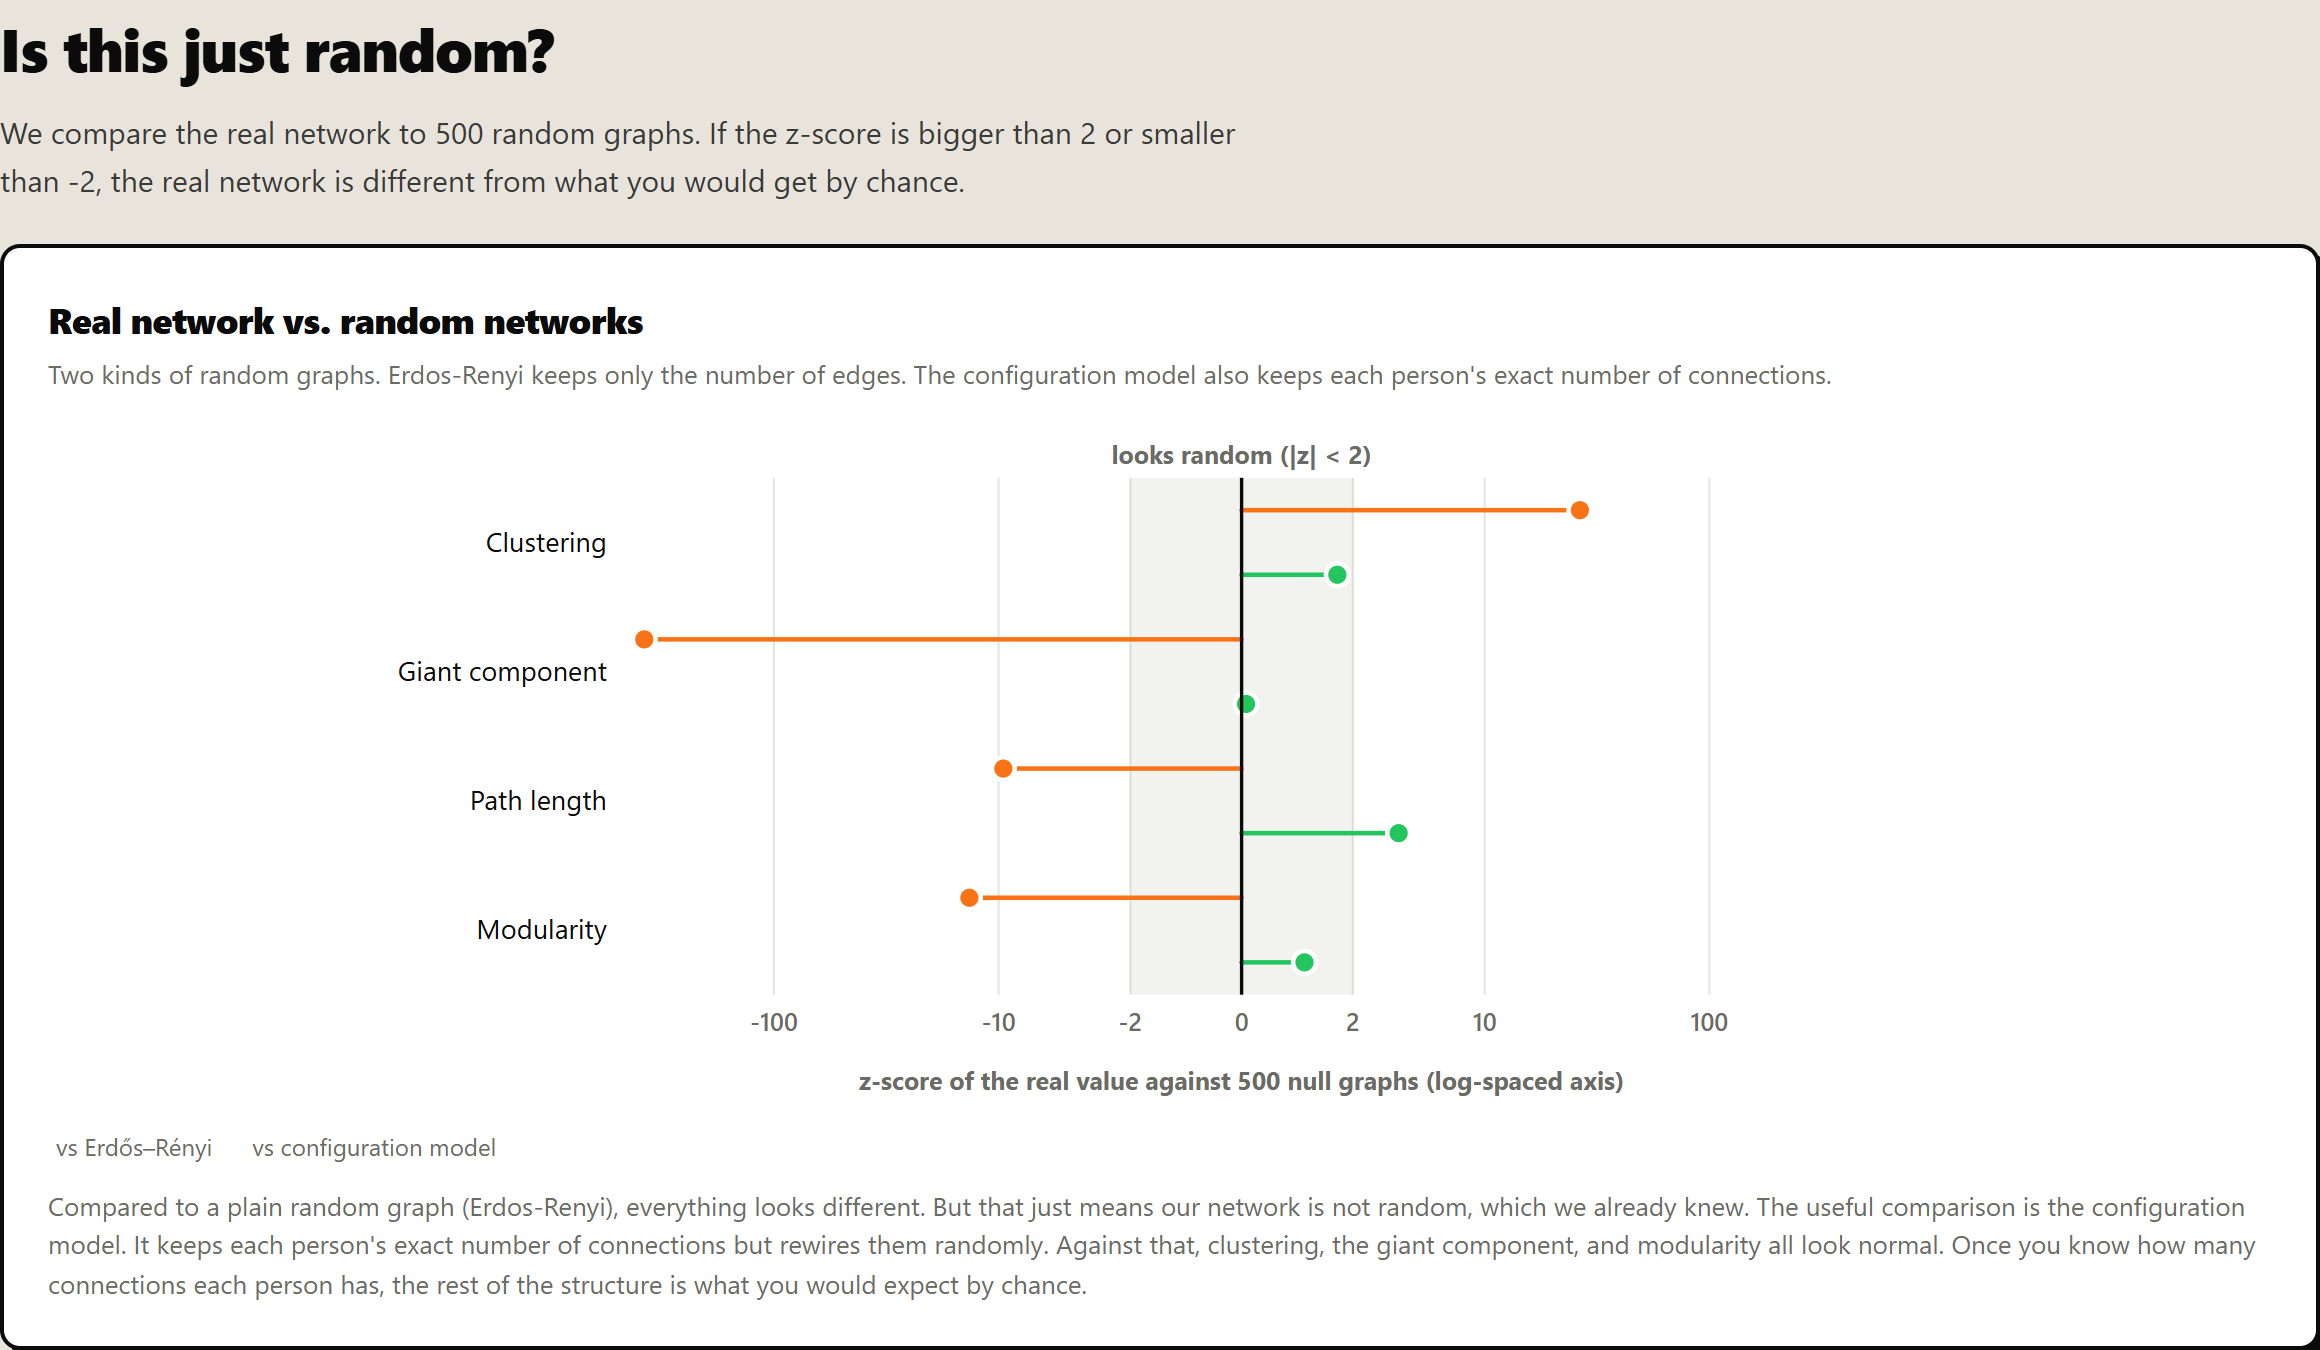
\includegraphics[width=0.86\linewidth]{../figures/dashboard/nullmodels.png}
  \caption{Null-model z-scores on a symmetric-log axis. The shaded band is the
  $|z|<2$ range that looks random. Erd\H{o}s--R\'enyi fails every measure. The
  configuration model matches clustering, giant component, and modularity.}
  \label{fig:null}
\end{figure}

\lab{Finding 5. The communities are real, but only at the fine grain.} A
permutation test shuffles the community labels 10{,}000 times with the group sizes
held fixed, then measures the opinion variance inside the groups. The p-value is
the fraction of shuffles that beat the real grouping.

\begin{table}[htbp]
\centering\small
\begin{tabular}{@{}lrrrr@{}}
\toprule
\sffamily\bfseries Features tested & \sffamily Observed & \sffamily Null mean &
\sffamily $z$ & \sffamily $p$ \\
\midrule
All 60 question scores & 0.4116 & 0.4592 & \gc{$-6.57$} & \gc{$<0.0001$} \\
4 topic means          & 0.0791 & 0.0839 & \rc{$-1.26$} & \rc{$0.108$} \\
\bottomrule
\end{tabular}
\caption{The same communities pass on the answers the graph was built from and
fail on the coarser topic averages.}
\label{tab:perm}
\end{table}

\begin{dash}
  \item On the 60 question scores the Louvain grouping is far tighter than chance
  ($z=-6.57$, $p<0.0001$).
  \item On the 4 topic means it is not distinguishable from random ($z=-1.26$,
  $p=0.108$).
  \item Louvain groups people by their detailed answer pattern, not by their
  broad position on the four topics. Two people in one community can differ on
  topic averages while answering the individual questions alike.
  \item The community-by-topic heatmap therefore \emph{describes} each group but
  does not \emph{define} it, and is not presented as a definition.
\end{dash}

\begin{figure}[htbp]
  \centering
  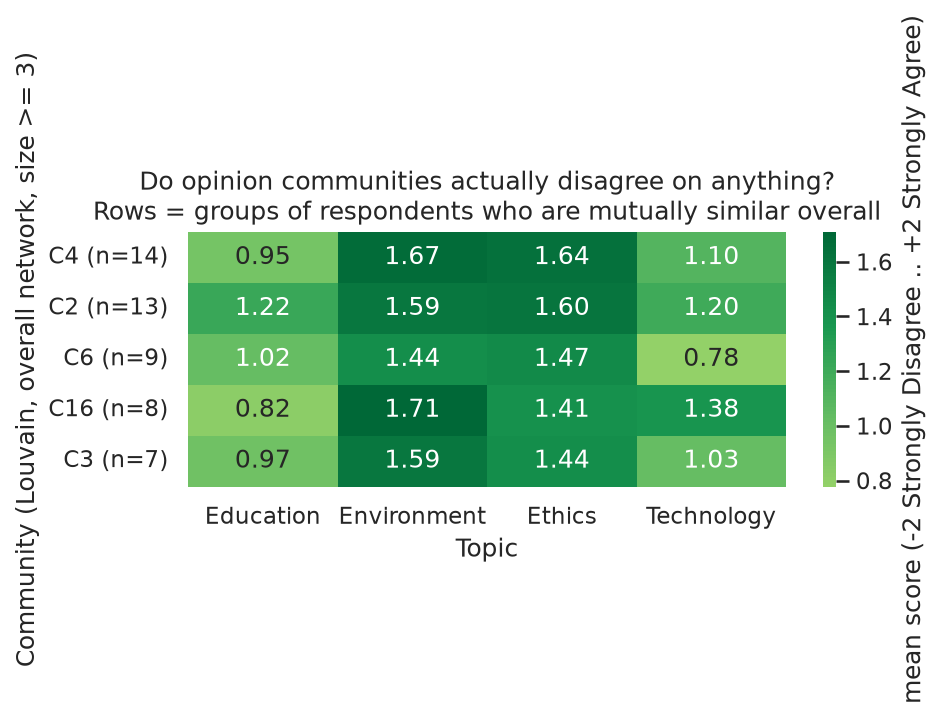
\includegraphics[width=0.54\linewidth]{../figures/community_topic_heatmap.png}
  \caption{Mean score of each large community, per topic. Every cell is positive.
  The communities raise or lower agreement rather than disagreeing.}
  \label{fig:heatmap}
\end{figure}

\lab{In summary:}
\begin{dash}
  \item The class is agreeable across all four topics, with no real factions.
  \item Low variance drives the apparent cohesion, so Technology and Education
  out-connect Ethics and Environment even with lower means.
  \item The connected core is a behaviour type, the uniform strong-agreement
  answerers, not a demographic or a topic camp.
  \item Centrality measures disagree about who matters, and that disagreement is
  itself a result.
  \item Ethics and Environment move together at a respondent-level $r=0.70$ and
  form one values axis. Technology and Education are nearly independent at
  $r=0.29$.
\end{dash}

% ============================================================
\section{Individual Contribution}

\begin{table}[htbp]
\centering\small
\begin{tabular}{@{}p{0.13\linewidth}p{0.81\linewidth}@{}}
\toprule
\sffamily\bfseries Member & \sffamily\bfseries Tasks completed \\
\midrule
\textbf{Aviral} &
Cleaned and interpreted the survey data. Built all five networks with cosine
similarity and the top-10\% cut. Ran the structural analysis: degree, clustering,
components, the four centralities, and the Louvain communities. Produced the
static figures. Found the topic-variance result and the centrality result. \\
\addlinespace
\textbf{Varun} &
Ran the dynamics and the spectral analysis. Ran the DeGroot average with the
Laplacian stability analysis. Computed the SIS epidemic threshold and its
simulation. Built the Erd\H{o}s--R\'enyi and configuration null models. Ran the
community permutation test and the edge-threshold sensitivity sweep. \\
\addlinespace
\textbf{Arihant} &
Built the self-contained interactive dashboard: hand-drawn charts, a node-link
view, all five networks, community and opinion colour, an isolate toggle, a
respondent lookup, and the dynamics and null-model panels. Exported the dashboard
data. Wrote this report and produced its figures. \\
\bottomrule
\end{tabular}
\caption{Individual contributions. The commit history matches this split.}
\label{tab:contrib}
\end{table}

\lab{Reproducibility:} everything in this report comes from the linked
repository. The pipeline runs as a fixed sequence of stages and writes its results
to disk, so no figure or table is computed by hand. The dashboard is a single HTML
file that opens in any browser with no server, no build step, and no network
access.

\end{document}
